\section{TODO: A preview of Constrained Optimization}
    \subsection{Subject to a Unit Vector}
    In some applications, we often need to find the maximum or minimum value of a quadratic form $Q(\B{x)}$ for $\B{x}$ in some specified set. For example,
    \begin{equation*}
        c = \underset{\lVert \B{x} \rVert = 1}{\argmin}\ Q({\B{x}})
    \end{equation*}
    
    \begin{figure}[ht]
    \centering
    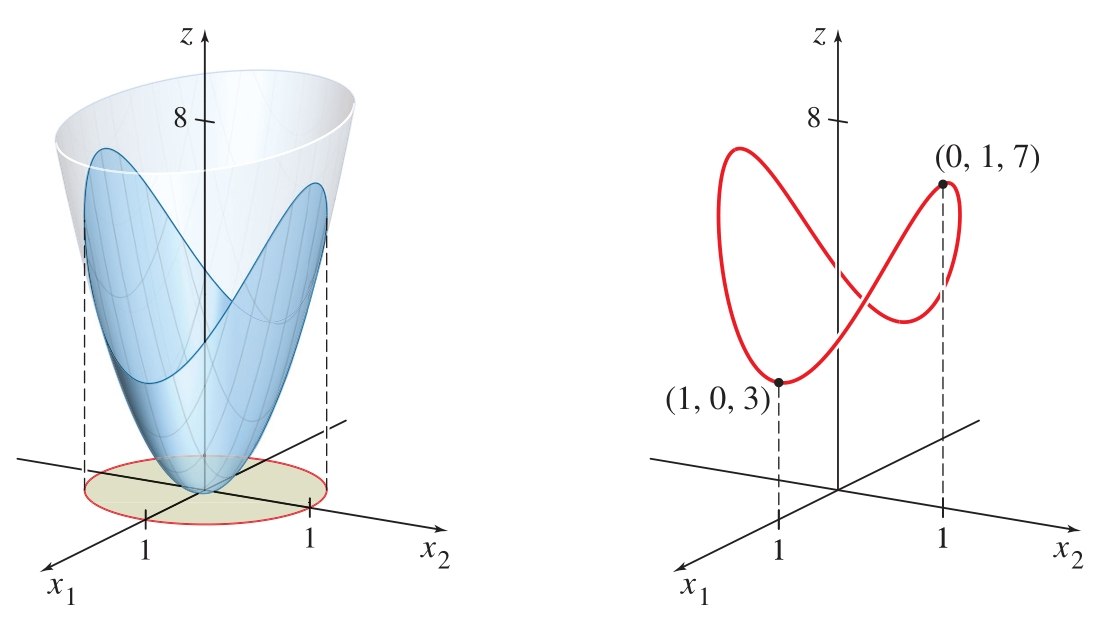
\includegraphics[width=0.6\textwidth]{images/constrained-1.jpg}
    \caption{$z = 3x_1^2 + 7x_2^2$ constrained on $x_1^2+x_2^2 = 1$}
   %\label{Find the principal axes.}
    \end{figure}

    \begin{Thm}\label{unit-opt}
        Given a quadratic form $Q(\B{x})$, and let $m = \underset{\lVert \B{x} \rVert = 1}{\argmin}\ Q({\B{x}})$ and $M = \underset{\lVert \B{x} \rVert = 1}{\argmax}\ Q({\B{x}})$. then 
        \begin{enumerate}
            \item $M$ is the greatest eigenvalue $\lambda_1$ of $A$
            \item $m$ is the least eigenvalue $\lambda_n$ of $A$.
        \end{enumerate}
        The value of $\quadratic{x}{A}$ is
        \begin{enumerate}
            \item $M$ when $\B{x}$ is a unit eigenvector $\B{u}_1$ corresponding to $\lambda_1$
            \item $m$ when $\B{x}$ is a unit eigenvector $\B{u}_m$ corresponding to $\lambda_n$
        \end{enumerate}
        \begin{proof}
            By the \cref{orthogonally-dianonalizable}, $A$ can be orthogonally diagonalized as $PDP^{-1}$, where either $P$ or $P^{-1}$ is an orthogonal matrix, thus preserving the length $\B{x}$. By \cref{change-of-variable}
            \begin{equation*}
                Q(\B{x}) = Q'(\B{y}) = \sum_{i = 1}^n \lambda_i y_i^2
            \end{equation*}
            where $\lambda$'s are arranged in descending order. The following inequality holds:
            \begin{align*}
                Q'(\B{y})\leq \lambda_1 \sum_{i = 1}^n y_i^2 = \lambda_1 \T{\B{y}}\B{y}
            \end{align*}
            where $\lambda_1$ is the largest eigenvalue of $A$. Let $\B{y}$ be $\B{e}_1$, a vector with the first entry being $1$ and the other being $0$. Then,
            \begin{equation*}
                \lambda_1 \T{\B{y}}\B{y} = \T{\B{e}_1} D\B{e}_1 
            \end{equation*}
            illustrates that $Q'(\B{y})$ reaches its maximum value when $\B{y} = \B{e}_1$, implying that $Q(\B{x})$ attains its maximum value when $\B{x} = P\B{e}_1 = \B{u}_1$. A similar method can be applied to prove its minimum value.
        \end{proof}
    \end{Thm}
    \begin{Thm}
        Given a quadratic form $Q(\B{x}) = \quadratic{x}{A}$, let $\lambda_1$ be the largest eigenvalue of $A$, and $\B{u}_1$ be the eigenvector corresponding to $\lambda_1$. then the maximum value of $Q$ subject to the following constrains:
        \begin{equation*}
            \T{\B{x}}\B{x} = 1,\quad \T{\B{x}}\B{u}_1 = 0
        \end{equation*} is the second greatest eigenvalue $\lambda_2$, and this maximum is attained when $\B{x}$ is an eigenvector $\B{u}_2$ corresponding to $\lambda_2$.
        \begin{Rem}
            Suppose that $A$ is orthogonally diagonalized as $PDP^{-1}$ with its eigenvalues arranged, in descending order, on the main diagonal of $D$. 
            If there are more constrains on $Q$:
            \begin{equation*}
                \T{\B{x}}\B{x} = 1,\quad \T{\B{x}}\B{u}_1 = 0,\quad \cdots, \T{\B{x}}\B{u}_{k - 1} = 0
            \end{equation*}
            then the maximum of $Q$ is attained at $\B{x} = \B{u}_k$ where $\B{u}_k$ is the eigenvector corresponding to the $k^{\text{th}}$ greatest eigenvalue.
        \end{Rem}
    \end{Thm}